\documentclass[aps,prd,onecolumn,11pt,nofootinbib]{revtex4-2}

% -------------------------------------------------------------
% PACKAGES
% -------------------------------------------------------------
\usepackage[utf8]{inputenc}
\usepackage[T1]{fontenc}
\usepackage{microtype}
\usepackage{amsmath,amssymb,amsthm}
\usepackage{bm}
\usepackage{mathtools}
\usepackage{graphicx}
\usepackage{booktabs}
\usepackage{array}
\usepackage{hyperref}
\usepackage[dvipsnames,svgnames,x11names]{xcolor}
\usepackage{lmodern}
\usepackage{tikz}

\hypersetup{
    colorlinks = true,
    linkcolor  = Blue,
    citecolor  = Blue,
    urlcolor   = Blue
}

% -------------------------------------------------------------
% MACROS
% -------------------------------------------------------------
\newcommand{\Aq}{\mathcal{A}(\theta;q)}
\newcommand{\phiq}{\phi(\theta;q)}

% -------------------------------------------------------------
% DOCUMENT START
% -------------------------------------------------------------
\begin{document}

\title{\bfseries A Scalar Diagnostic for Empirical Score Alignment on Fisher Manifolds}

\author{Isaid Cornejo}
\email{isaidcor@gmail.com}
\affiliation{Information Physics Institute}
\altaffiliation{ORCID: 0009-0008-5550-9716}

\date{\today}

\begin{abstract}
The Fisher--Rao metric provides the canonical geometric structure on statistical
manifolds \cite{Fisher1922,Rao1945,AmariNagaoka2000}, yet empirical data often
induce strong deviations from this geometry. Such deviations manifest through
heavy-tailed spectra, dominant outlier modes, and effective dimensionality
collapse in modern statistical models and neural networks
\cite{Papyan2019,Sagun2016}. Despite their ubiquity, existing metrics for
quantifying these effects (e.g., effective rank, participation ratio, spectral
decay indices) lack reparametrization invariance and do not directly compare
empirical sensitivity to the intrinsic geometric baseline.

We introduce a coordinate-free scalar diagnostic that measures the empirical
deformation of Fisher geometry:
\[
\mathcal{A}(\theta;q) = G^{ij}(\theta)\,\big(C_{ij}(\theta;q)-G_{ij}(\theta)\big),
\]
together with its rectified amplitude
\[
\phi(\theta;q) = \max\{\sqrt{\mathcal{A}},\,0\}.
\]
We show that the alignment operator $H = G^{-1}C$ is diagonalizable with real
non-negative eigenvalues $\lambda_i$, and that
$\mathcal{A} = \sum_i (\lambda_i - 1)$. Thus $\mathcal{A}$ provides a signed,
invariant summary of empirical reinforcement ($\lambda_i>1$) and suppression
($\lambda_i<1$), while $\phi$ isolates the excess-alignment sector.

We validate the diagnostic across exponential families (Gaussian, Laplace)
\cite{Brown1986}, a Gaussian mixture model \cite{McLachlanPeel2000}, and a
trained neural network on MNIST \cite{LeCun1998}, demonstrating that
$\mathcal{A}$ captures equilibrium, suppression, and strong empirical
reinforcement in a unified scalar signature. Reproducible code and figures are
provided online.

\end{abstract}

\maketitle

% -------------------------------------------------------------
% MAIN SECTIONS
% -------------------------------------------------------------
\section{Introduction}

The Fisher--Rao metric endows parametric statistical models with a canonical
Riemannian structure that reflects infinitesimal statistical distinguishability
\cite{Fisher1922,Rao1945,AmariNagaoka2000,Amari2016}. Its geometric
interpretation underlies classical asymptotic theory, natural gradient
optimization \cite{Amari1998,Martens2014}, exponential-family structure
\cite{Brown1986,WainwrightJordan2008}, and the analysis of likelihood curvature
in information geometry.

In practice, empirical data seldom match the model distribution exactly.
Whenever the data-generating distribution $q(x)$ differs from the model
$p(x|\theta)$, empirical score statistics become anisotropic, leading to
heavy-tailed empirical Fisher matrices, dominant outlier eigenvalues, and
effective dimensionality collapse. These phenomena are now well documented in
high-dimensional models and deep networks
\cite{Papyan2019,Sagun2016,Laurent2018,Nakkiran2020}.

Despite extensive spectral evidence, there remains no single, intrinsic,
reparametrization-invariant scalar quantity that measures how empirical
sensitivity deviates from the Fisher baseline. Existing notions of effective
dimensionality (e.g., participation ratio, effective rank, spectral entropy) are
useful but do not compare empirical covariance to the intrinsic geometric
expectation imposed by Fisher--Rao structure.

\textbf{This work introduces a coordinate-free scalar diagnostic}:
\[
\mathcal{A}(\theta;q) = \mathrm{Tr}\!\left(G^{-1}C\right) - D,
\]
together with a rectified amplitude
\[
\phi(\theta;q) = \max\{\sqrt{\mathcal{A}},0\}.
\]

We show that this diagnostic:
\begin{itemize}
    \item measures the total empirical deviation from Fisher geometry,
    \item admits a spectral form $\mathcal{A} = \sum_i (\lambda_i - 1)$,
    \item distinguishes reinforcement from suppression through its sign,
    \item collapses high-dimensional spectral behavior into a single invariant.
\end{itemize}

The remainder of the paper is organized as follows.
Section~\ref{sec:background} reviews Fisher geometry and empirical covariance.
Section~\ref{sec:diagnostic} defines the alignment tensor and the scalar
diagnostic. Section~\ref{sec:spectral} develops the spectral representation.
Section~\ref{sec:regimes} characterizes equilibrium, suppression, and excess
alignment. Section~\ref{sec:experiments} presents empirical demonstrations.
Section~\ref{sec:discussion} discusses implications and limitations, and
Section~\ref{sec:conclusion} concludes.

\section{Background}
\label{sec:background}

Let $p(x|\theta)$ be a regular parametric statistical model with parameter
$\theta \in \Theta \subset \mathbb{R}^D$. The score is defined as
\[
v_i(x|\theta) = \partial_i \log p(x|\theta),
\]
and the Fisher--Rao metric is
\[
G_{ij}(\theta) = \mathbb{E}_{p}[v_i v_j]
\]
as introduced in the foundational works of Fisher and Rao
\cite{Fisher1922,Rao1945} and formalized in modern information geometry
\cite{AmariNagaoka2000,Amari2016}.

When empirical expectations are taken with respect to a distribution $q(x)$ that
differs from $p(x|\theta)$, the empirical score covariance,
\[
C_{ij}(\theta;q) = \mathbb{E}_{q}[v_i v_j],
\]
generally deviates from the Fisher metric. This mismatch produces anisotropic
empirical sensitivity.

In modern statistical models---particularly deep networks---empirical Fisher
matrices often exhibit:
\begin{itemize}
    \item heavy-tailed spectral decay,
    \item dominant outlier eigenvalues,
    \item effective dimensionality collapse,
\end{itemize}
phenomena that have been extensively documented in recent deep learning
literature \cite{Papyan2019,Sagun2016,Laurent2018,Nakkiran2020}.

These effects motivate the need for principled, invariant diagnostics capable of
characterizing empirical deviation from Fisher geometry.

\section{The Alignment Tensor and Scalar Diagnostic}
\label{sec:diagnostic}

This section introduces the core geometric objects used throughout the paper:
the empirical-alignment tensor, the scalar deviation diagnostic
$\mathcal{A}(\theta;q)$, and its rectified amplitude $\phi(\theta;q)$.
Together, these quantify how empirical sensitivity departs from the intrinsic
Fisher--Rao structure \cite{AmariNagaoka2000,Amari2016}.

% -------------------------------------------------------------
\subsection{Empirical Score Covariance}

Empirical expectations with respect to the data distribution $q(x)$ define the
empirical score covariance:
\begin{equation}
C_{ij}(\theta;q) = \mathbb{E}_{q}[\,v_i v_j\,].
\end{equation}
In general $C_{ij}(\theta;q)$ and $G_{ij}(\theta)$ need not coincide unless
$q=p$, and even then equality may fail outside minimal exponential families
\cite{Brown1986,WainwrightJordan2008}.

The discrepancy between these two tensors captures the geometric deformation
induced by the data.

% -------------------------------------------------------------
\subsection{The Alignment Tensor}

We define the empirical-alignment tensor
\begin{equation}
\Delta_{ij}(\theta;q) = C_{ij}(\theta;q) - G_{ij}(\theta).
\end{equation}

Interpretationally:
\begin{itemize}
    \item $\Delta_{ij} = 0$ indicates Fisher-equivalent sensitivity.
    \item Positive eigenvalues of $\Delta$ correspond to reinforcement
    (empirical variance exceeding the Fisher baseline).
    \item Negative eigenvalues correspond to suppression.
\end{itemize}

Thus $\Delta_{ij}$ encodes direction-wise deviations of empirical sensitivity.

% -------------------------------------------------------------
\subsection{The Scalar Diagnostic}
\label{sec:scalar}

To obtain an invariant, coordinate-free quantity, we contract the alignment
tensor with the inverse Fisher metric:
\begin{equation}
\mathcal{A}(\theta;q)
    := G^{ij}(\theta)\,\Delta_{ij}(\theta;q)
    = \mathrm{Tr}\!\left(G^{-1} C\right) - D.
\end{equation}
\footnote{
The equivalence between the contractions 
$G^{ij}(C_{ij}-G_{ij})$ and $\mathrm{Tr}(G^{-1}C)-D$
follows from the identity $G^{ij}G_{ij} = \delta^{i}_{\,i} = D$,
which states that the trace of the Fisher metric equals the
dimension of the parameter space. This holds in any coordinate
system and does not assume a special parametrization.
}

This scalar diagnostic has three essential properties:
\begin{itemize}
    \item \textbf{Reparametrization invariance}: it transforms as a scalar under
    smooth parameter transformations.
    \item \textbf{Signed structure}: $\mathcal{A}>0$ indicates net reinforcement,
    whereas $\mathcal{A}<0$ indicates net suppression.
    \item \textbf{Nontriviality}: $\mathcal{A}=0$ does not imply $C_{ij}=G_{ij}$
    unless the model satisfies strict exponential-family regularity
    \cite{Brown1986}.
\end{itemize}

% -------------------------------------------------------------
\subsection{Rectified Excess-Alignment Amplitude}

In many settings only the \emph{excess-alignment sector} is of interest—namely
the directions along which empirical sensitivity exceeds the Fisher baseline.
We therefore introduce the rectified amplitude:
\begin{equation}
\phi(\theta;q) = \max\{\sqrt{\mathcal{A}(\theta;q)},\,0\}.
\end{equation}

By construction:
\[
\phi = 0 
\quad\Longleftrightarrow\quad
\mathcal{A} \le 0.
\]

The quantity $\phi$ behaves analogously to an amplitude that captures the total
strength of empirical reinforcement across all Fisher-orthonormal directions.
The square-root scaling has a natural interpretation: since 
$\mathcal{A} = \sum_i(\lambda_i - 1)$ aggregates deviations additively, taking
$\sqrt{\mathcal{A}}$ produces a Fisher-normalized magnitude rather than an
energy-like sum. In this sense, $\phi$ acts as an amplitude associated with the
subspace where $\lambda_i > 1$, providing a more interpretable measure of
excess alignment intensity.

% -------------------------------------------------------------
\subsection{Signed Interpretation}

The sign of $\mathcal{A}$ carries direct geometric meaning:
\begin{align*}
\mathcal{A} > 0: &\quad \text{net empirical reinforcement}, \\
\mathcal{A} = 0: &\quad \text{Fisher-equivalent sensitivity}, \\
\mathcal{A} < 0: &\quad \text{net empirical suppression}.
\end{align*}

Reinforcement corresponds to directions in which empirical curvature exceeds
Fisher curvature, while suppression identifies damped or collapsed empirical
modes.

These features become especially transparent through the spectral
representation developed in Section~\ref{sec:spectral}.


\section{Spectral Structure of the Alignment Operator}
\label{sec:spectral}

The scalar diagnostic $\mathcal{A}(\theta;q)$ becomes fully transparent when
expressed through a natural mixed tensor that compares empirical and geometric
sensitivity \emph{direction by direction}. This section develops the spectral
structure of that operator and establishes the key identity
\[
\mathcal{A} = \sum_{i=1}^D (\lambda_i - 1),
\]
which provides a complete and invariant summary of empirical deformation.

% -------------------------------------------------------------
\subsection{The Alignment Operator}

Raising one index of the empirical covariance with the inverse Fisher metric
defines the $(1,1)$ alignment operator:
\begin{equation}
H^i_{\;j}(\theta;q)
    := G^{ik}(\theta)\,C_{kj}(\theta;q).
\label{eq:H_def}
\end{equation}

Using the decomposition $C_{ij} = G_{ij} + \Delta_{ij}$, we obtain
\begin{equation}
H^i_{\;j} = \delta^i_{\;j} + G^{ik}\Delta_{kj},
\label{eq:H_decomposition}
\end{equation}
so that:
\begin{itemize}
    \item $H = I$ under Fisher-equilibrium sensitivity,
    \item deviations from the identity encode empirical alignment,
    \item reinforcement and suppression manifest as eigenvalues above or below~1.
\end{itemize}

Although $H$ need not be symmetric, it inherits strong spectral structure from
the positive definiteness of the Fisher metric
\cite{AmariNagaoka2000,Amari2016}.

% -------------------------------------------------------------
\subsection{Diagonalizability and Symmetric Surrogate}

Because $G$ is positive definite, it admits a symmetric square root $G^{1/2}$
and its inverse $G^{-1/2}$ \cite{AmariNagaoka2000}. Writing
\[
H = G^{-1}C
\qquad\Longrightarrow\qquad
H \sim G^{-1/2} C\, G^{-1/2},
\]
we see that $H$ is similar to the symmetric matrix
$G^{-1/2} C\, G^{-1/2}$.

Consequences:
\begin{itemize}
    \item all eigenvalues of $H$ are real and non-negative,
    \item $H$ is diagonalizable,
    \item the spectrum of $H$ equals that of the symmetric surrogate.
\end{itemize}

Thus the empirical sensitivity deformation can be studied through a symmetric
operator without altering the underlying geometry.

% -------------------------------------------------------------
\subsection{Eigenvalues as Sensitivity Ratios}

Let $\lambda_1,\ldots,\lambda_D$ denote the eigenvalues of $H$, with eigenvectors
$u^{(i)}$ normalized with respect to the Fisher metric:
\[
G^{ij} u_i^{(k)} u_j^{(k)} = 1.
\]

Inserting these eigenvectors into the relation $Hu = \lambda u$ yields:
\begin{equation}
\lambda
    = u^{i} C_{ij} u^{j},
\label{eq:lambda_interpretation}
\end{equation}
so each eigenvalue measures the empirical variance of the score \emph{relative to}
the Fisher--Rao expectation in that direction.

Interpretation:
\begin{itemize}
    \item $\lambda_i > 1$ \quad reinforced empirical sensitivity,
    \item $\lambda_i < 1$ \quad suppressed empirical sensitivity,
    \item $\lambda_i = 1$ \quad Fisher-equivalent sensitivity.
\end{itemize}

The spectrum of $H$ therefore gives a direction-wise decomposition of empirical
alignment on the statistical manifold.

% -------------------------------------------------------------
\subsection{Trace Identity and the Scalar Diagnostic}

Taking the trace of the decomposition in
Eq.~\eqref{eq:H_decomposition} immediately gives
\[
\mathrm{Tr}(H) = D + \mathrm{Tr}(G^{-1}\Delta).
\]

Hence
\begin{equation}
\mathcal{A}(\theta;q)
    = \mathrm{Tr}(G^{-1}C) - D
    = \mathrm{Tr}(H) - D
    = \sum_{i=1}^D (\lambda_i - 1).
\label{eq:trace_identity}
\end{equation}

This establishes that $\mathcal{A}$ aggregates the total empirical deviation of
$H$ from the identity and that the rectified amplitude
\[
\phi = \max\{\sqrt{\mathcal{A}},0\}
\]
captures the \emph{total strength of excess alignment}.

% -------------------------------------------------------------
\subsection{Finite-Sample Resolution and Minimal Coherent Alignment}

The scalar diagnostic
\begin{equation}
\mathcal{A}(\theta;q) = \mathrm{Tr}(G^{-1}C) - D
\end{equation}
is defined exactly and invariantly at the population level. In empirical
settings, however, all expectations entering the empirical score covariance
$C_{ij}$ are estimated from a finite sample of size $N$. As a consequence, even
under perfect Fisher equilibrium ($q=p$), the empirical alignment operator
\begin{equation}
H = G^{-1}C
\end{equation}
does not coincide exactly with the identity, but exhibits spectral fluctuations
arising purely from finite-sample effects.

Under standard regularity assumptions and for fixed parameter dimension, the
eigenvalues $\lambda_i$ of $H$ fluctuate around unity with typical deviations of
order
\begin{equation}
\lambda_i - 1 = \mathcal{O}(N^{-1/2}),
\end{equation}
independently of any genuine geometric misalignment. Deviations at this scale
therefore do not correspond to resolvable empirical structure, but instead
reflect statistical uncertainty in the estimation of score covariances.

This observation implies the existence of a \emph{minimal geometric resolution
scale} $\epsilon_N$, below which departures from Fisher equilibrium are not
operationally meaningful. We therefore distinguish between \emph{formal
alignment}, captured by the scalar diagnostic $\mathcal{A}$, and
\emph{resolvable coherent alignment}, defined by excluding spectral deviations
that lie within the Fisher--geometric noise floor. Importantly,
$\mathcal{A}_{\min}$ is not a geometric invariant, but an operational diagnostic
whose definition depends explicitly on finite-sample resolution.

Concretely, we introduce the minimally resolvable excess-alignment diagnostic
\begin{equation}
\mathcal{A}_{\min}(\theta;q)
\;=\;
\sum_{\lambda_i > 1 + \epsilon_N} (\lambda_i - 1),
\qquad
\epsilon_N \sim \mathcal{O}(N^{-1/2}),
\end{equation}
which isolates only those eigenmodes whose empirical reinforcement exceeds the
finite-sample resolution threshold. Only such modes are interpreted as carrying
coherent geometric alignment.

This refinement does not modify the underlying construction of the alignment
operator, nor the definition of the scalar diagnostic $\mathcal{A}$ itself.
Rather, it makes explicit the empirical resolution limit inherent to finite
data. In particular, the condition $\mathcal{A}_{\min}=0$ should be interpreted
as the absence of \emph{resolvable excess alignment}, which may arise either from
true Fisher equilibrium or from empirical deviations that remain below the
finite-sample noise floor.

For empirical interpretation, it is often convenient to define a corresponding
\emph{resolvable coherent amplitude}
\begin{equation}
\phi_{\mathrm{res}}(\theta)
\;=\;
\max\{\sqrt{\mathcal{A}_{\min}(\theta;q)},\,0\},
\end{equation}
which provides a finite-sample--robust measure of the intensity of coherent
empirical reinforcement. This quantity plays an interpretive role analogous to
the formal amplitude $\phi=\max\{\sqrt{\mathcal{A}},0\}$, but suppresses
artificial inflation due to the accumulation of sub-threshold fluctuations, a
particularly relevant effect in high-dimensional models such as deep neural
networks.

Throughout this work, empirical results are therefore interpreted with respect
to both the formal diagnostic $\mathcal{A}$ and its resolvable counterparts
$\mathcal{A}_{\min}$ and $\phi_{\mathrm{res}}$. This distinction is essential in
heterogeneous or multi-scale systems, where genuine structural reinforcement may
coexist with equally strong suppression across different directions of parameter
space, yet only reinforced modes that exceed the finite-sample resolution
threshold contribute to resolvable coherent alignment.

% -------------------------------------------------------------
\subsection{Relation to Dimensionality Measures}

Although related to classical measures of effective dimensionality such as the
participation ratio and effective rank, the diagnostic $\mathcal{A}$ differs in
three key ways:
\begin{itemize}
    \item it compares empirical sensitivity directly against the Fisher baseline,
    \item it is signed, distinguishing suppression and reinforcement,
    \item it is a scalar invariant under reparametrization.
\end{itemize}

Thus $\mathcal{A}$ offers a complementary perspective to spectral summaries
commonly used in high-dimensional statistics and deep learning
\cite{Papyan2019,Sagun2016,Laurent2018,Nakkiran2020}.

\section{Alignment Regimes}
\label{sec:regimes}

The spectrum of the alignment operator $H = G^{-1}C$ naturally partitions the
behavior of empirical sensitivity into three fundamental regimes:
\emph{equilibrium}, \emph{sup\-pression}, and \emph{excess alignment}. Each regime
corresponds to a distinct empirical deformation of Fisher--Rao geometry and has
clear geometric and statistical interpretation.

We summarize these regimes below before turning to empirical demonstrations.

\begin{figure}[t]
\centering

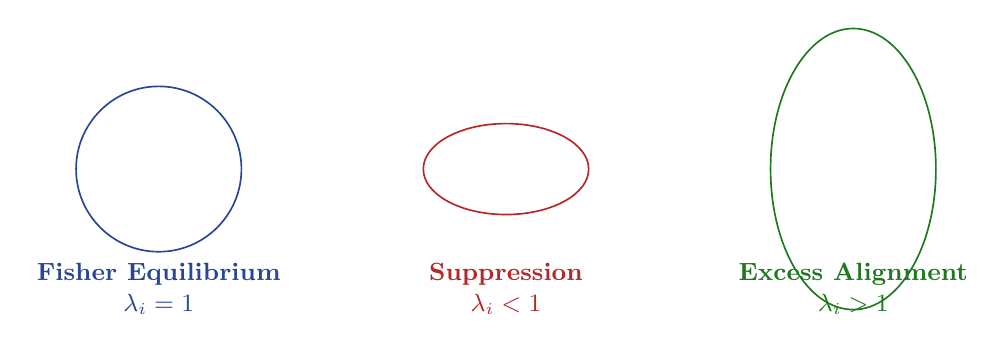
\begin{tikzpicture}[scale=1.05]

    % Colors in a more professional physics palette
    \definecolor{eqcol}{RGB}{40,70,150}
    \definecolor{supcol}{RGB}{180,40,40}
    \definecolor{excol}{RGB}{30,120,30}

    % Common text style
    \tikzset{
        reglabel/.style={font=\small\bfseries, align=center}
    }

    % ============== Fisher equilibrium (circle) ==============
    \begin{scope}[xshift=0cm]
        \draw[semithick, eqcol] (0,0) circle (1cm);
        \node[eqcol, reglabel] at (0,-1.45)
            {Fisher Equilibrium\\$\lambda_i = 1$};
    \end{scope}

    % ================== Suppression ellipse ==================
    \begin{scope}[xshift=4.2cm]
        \draw[semithick, supcol] (0,0) ellipse (1cm and 0.55cm);
        \node[supcol, reglabel] at (0,-1.45)
            {Suppression\\$\lambda_i < 1$};
    \end{scope}

    % ================= Excess Alignment ellipse ==============
    \begin{scope}[xshift=8.4cm]
        \draw[semithick, excol] (0,0) ellipse (1cm and 1.7cm);
        \node[excol, reglabel] at (0,-1.45)
            {Excess Alignment\\$\lambda_i > 1$};
    \end{scope}

\end{tikzpicture}

\caption{
Geometric regimes of empirical alignment on a Fisher manifold.
Equilibrium corresponds to isotropic curvature ($\lambda_i=1$),
suppression reflects contraction of sensitivity along one or more axes
($\lambda_i<1$), and excess alignment corresponds to expansion beyond
the Fisher baseline ($\lambda_i>1$).
}
\label{fig:alignment-regimes}
\end{figure}


% -------------------------------------------------------------
\subsection{Fisher Equilibrium}

A model is in Fisher equilibrium at $\theta$ when
\[
\lambda_i(\theta;q) = 1 \quad \text{for all } i.
\]
In this regime, empirical score covariance matches the geometric expectation set
by the Fisher metric. The alignment tensor vanishes,
\[
\Delta_{ij} = 0,
\qquad
\mathcal{A} = 0,
\qquad
\phi = 0,
\]
and the empirical sensitivity landscape is isotropic in Fisher-orthonormal
coordinates.

This regime occurs when $q=p$ in minimal exponential families
\cite{Brown1986,WainwrightJordan2008} or when empirical and model curvature
coincide despite mild model misspecification. Gaussian families (with mean and
variance parameters) provide canonical examples.

% -------------------------------------------------------------
\subsection{Suppression Regime}

The suppression regime corresponds to
\[
\lambda_i < 1 \quad \text{for one or more eigenvalues}.
\]
Here empirical variance falls \emph{below} the Fisher--Rao baseline, indicating
that the data distribution $q$ concentrates sensitivity into a lower-dimensional
tangent subspace than predicted by the model.

Key signatures:
\[
\mathcal{A} < 0,
\qquad
\phi = 0,
\]
reflecting a net contraction of empirical sensitivity.

Suppression manifests in models with heavy-tailed likelihood structure, sharp
modes, or symmetry-induced collapse. The Laplace family provides a simple
example: even under $q=p$, empirical curvature does not match Fisher curvature,
yielding slight suppression \cite{LaplaceDistribution}.

Geometrically, suppression corresponds to a flattening of the empirical local
quadratic structure relative to the intrinsic Fisher geometry.

% -------------------------------------------------------------
\subsection{Excess Alignment}

Excess alignment occurs when
\[
\exists\, i : \lambda_i > 1,
\]
and is characterized by empirical reinforcement along one or more
Fisher-orthonormal directions.

In this regime:
\[
\mathcal{A} > 0,
\qquad
\phi = \sqrt{\mathcal{A}}.
\]

Large outlier eigenvalues reflect strong anisotropy in empirical sensitivity,
where $q$ emphasizes fluctuations aligned with specific directions of the tangent
space. Gaussian mean-shift perturbations yield mild excess alignment; neural
networks often display extreme instances, with $\lambda_{\max} \gg 1$ indicating
dominant reinforcement modes \cite{Sagun2016,Papyan2019,Laurent2018}.

Geometrically, excess alignment corresponds to an empirical reshaping of the
local geometry into a directionally stretched structure relative to the Fisher
metric.

% -------------------------------------------------------------
\subsection{Mixed Regimes and Directional Structure}

In many practical cases, empirical spectra contain both suppressed and reinforced
directions:
\[
\lambda_{i_1} < 1,\qquad
\lambda_{i_2} > 1.
\]

Such mixed regimes occur frequently in:
\begin{itemize}
    \item misspecified models,
    \item mixture models,
    \item deep networks,
    \item hierarchical generative models.
\end{itemize}

The scalar diagnostic $\mathcal{A}$ measures the \emph{net} deviation across all
directions, while the full spectrum reveals the balance between reinforcement and
suppression.

% -------------------------------------------------------------
\subsection{Summary}

The three alignment regimes encode qualitatively different empirical geometric
behaviors:

\begin{table}[h!]
\centering
\begin{tabular}{ccp{0.48\textwidth}<{\raggedright\arraybackslash}}
\toprule
\textbf{Regime} & \textbf{Scalar Signature} & \textbf{Interpretation} \\
\midrule

Equilibrium & $\mathcal{A}=0$ &
Empirical curvature matches the Fisher expectation. \\

Suppression & $\mathcal{A}<0$ &
Empirical sensitivity is contracted relative to the Fisher baseline. \\

Excess Alignment & $\mathcal{A}>0$ &
Empirical reinforcement; increased anisotropy relative to Fisher geometry. \\

\bottomrule
\end{tabular}
\end{table}

These regimes will be illustrated concretely through empirical experiments in
Section~\ref{sec:experiments}.

\section{Empirical Validation Across Statistical Models}
\label{sec:experiments}

This section presents the empirical behavior of the scalar diagnostic
$\mathcal{A}(\theta;q)$ and its rectified amplitude $\phi(\theta;q)$ across four
families of models: Gaussian, Laplace, Gaussian mixtures, and a trained neural
network on MNIST. Each experiment follows the same computational pipeline:

\begin{enumerate}
    \item Compute the Fisher information matrix $G$.
    \item Compute the empirical covariance $C$ under the data distribution $q$.
    \item Form the Fisher-normalized operator
    \[
        H = G^{-1/2} C\, G^{-1/2},
    \]
    which is symmetric and positive semidefinite.
    \item Compute its eigenvalues $\lambda_i$.
    \item Evaluate the scalar diagnostic
    \[
        \mathcal{A} = \sum_{i=1}^D (\lambda_i - 1),
        \qquad
        \phi = \max\{\sqrt{\mathcal{A}},0\}.
    \]
\end{enumerate}

All experiments were generated using the reproducible suite in
\texttt{src/experiments/}, with figures automatically produced via:

\begin{verbatim}
python -m src.generate_figures
\end{verbatim}

The figures included below correspond exactly to the outputs stored in\\
\texttt{paper/figures/generated/}.

% -------------------------------------------------------------
\subsection{Gaussian Family: Equilibrium and Mean-Shift Misalignment}

The Gaussian model provides the simplest instance of Fisher equilibrium and
controlled deviation from it. Under $q=p$, the empirical covariance matches the
Fisher metric, yielding eigenvalues $\lambda_i \approx 1$ and thus
$\mathcal{A} \approx 0$.

\begin{figure}[H]
\centering
\includegraphics[width=0.70\linewidth]{../figures/generated/gaussian_equilibrium.png}
\caption{
Eigenvalue spectrum of the alignment operator for the Gaussian model under
Fisher equilibrium. Both eigenvalues satisfy $\lambda_i \approx 1$, producing
$\mathcal{A}\approx 0$ and $\phi=0$.
}
\label{fig:gaussian_eq}
\end{figure}

A simple mean shift induces asymmetric deformation of empirical sensitivity:
one direction becomes reinforced ($\lambda>1$) while the other is suppressed
($\lambda<1$). This produces $\mathcal{A}>0$ and a nonzero coherence amplitude.

\begin{figure}[H]
\centering
\includegraphics[width=0.70\linewidth]{../figures/generated/gaussian_misalignment.png}
\caption{
Gaussian misalignment via mean-shift. One eigenvalue is reinforced
($\lambda\approx 5$) while the other is suppressed, yielding
$\mathcal{A}>0$ and $\phi>0$.
}
\label{fig:gaussian_mis}
\end{figure}

% -------------------------------------------------------------
\subsection{Laplace Family: Structural Suppression}

The Laplace model is not a minimal exponential family, so even under $q=p$ the
empirical covariance deviates slightly from the Fisher metric
\cite{LaplaceDistribution}. This produces mild suppression ($\lambda_i < 1$) and
therefore $\mathcal{A}<0$.

\begin{figure}[H]
\centering
\includegraphics[width=0.70\linewidth]{../figures/generated/laplace_equilibrium.png}
\caption{
Laplace equilibrium. Even when $q=p$, the non-exponential-family structure
induces $\lambda_i < 1$ and $\mathcal{A}<0$, reflecting structural suppression.
}
\label{fig:laplace_eq}
\end{figure}

Under a shifted data distribution, both eigenvalues fall further below~1,
demonstrating clear global suppression and vanishing coherence amplitude:
$\phi=0$.

\begin{figure}[H]
\centering
\includegraphics[width=0.70\linewidth]{../figures/generated/laplace_misalignment.png}
\caption{
Laplace misalignment. Both eigenvalues satisfy $\lambda_i<1$, yielding
$\mathcal{A}<0$ and $\phi=0$, characteristic of a global suppression regime.
}
\label{fig:laplace_mis}
\end{figure}

% -------------------------------------------------------------
\subsection{Gaussian Mixture Model: Multimodal Reinforcement}

Gaussian mixtures introduce multimodality, leading to anisotropic empirical
curvature and mild outlier eigenvalues even under equilibrium conditions
\cite{McLachlanPeel2000}.

\begin{figure}[H]
\centering
\includegraphics[width=0.70\linewidth]{../figures/generated/gmm_equilibrium.png}
\caption{
GMM equilibrium. Small deviations around $\lambda_i \approx 1$ arise from
sampling variability and multimodal structure, with $\mathcal{A}\approx 0$.
}
\label{fig:gmm_eq}
\end{figure}

When the mixture is misaligned relative to the data, the empirical covariance
acquires clear reinforcement modes ($\lambda>1$) while other directions remain
suppressed, producing a net positive scalar diagnostic.

\begin{figure}[H]
\centering
\includegraphics[width=0.70\linewidth]{../figures/generated/gmm_misalignment.png}
\caption{
GMM misalignment. Multimodality induces reinforced directions
($\lambda>1$) and suppressed ones ($\lambda<1$), yielding $\mathcal{A}>0$.
}
\label{fig:gmm_mis}
\end{figure}

% -------------------------------------------------------------
\subsection{Neural Network on MNIST: Strong Empirical Anisotropy}

A fully connected network trained on MNIST \cite{LeCun1998} exhibits a
dramatically anisotropic alignment spectrum. The largest eigenvalue satisfies
$\lambda_{\max} \gg 1$, indicating extremely reinforced empirical curvature.
Most remaining eigenvalues collapse near zero, reflecting effective
dimensionality reduction \cite{Sagun2016,Papyan2019,Laurent2018}.

\begin{figure}[H]
\centering
\includegraphics[width=0.75\linewidth]{../figures/generated/mnist_alignment.png}
\caption{
Alignment spectrum of a trained MNIST MLP. The presence of a large outlier
eigenvalue ($\lambda_{\max} \gg 1$) indicates strong empirical reinforcement,
while the bulk collapses toward~0. This produces a large positive scalar
diagnostic $\mathcal{A}$ and a correspondingly strong coherence amplitude.
}
\label{fig:mnist}
\end{figure}

% -------------------------------------------------------------
\subsection{Summary}

Across all tested families—Gaussian, Laplace, mixture models, and neural
networks—the scalar diagnostic $\mathcal{A}$ and its rectified amplitude
$\phi$ accurately capture the empirical deformation of Fisher geometry:

\begin{itemize}
    \item $\mathcal{A} \approx 0$ under Fisher equilibrium,
    \item $\mathcal{A} < 0$ in structural or global suppression regimes,
    \item $\mathcal{A} > 0$ when empirical reinforcement emerges,
    \item large $\mathcal{A}$ in deep models with strong curvature outliers.
\end{itemize}

A consolidated numerical summary is provided in the table at the end of the
paper.

\section{Discussion}
\label{sec:discussion}

The scalar diagnostic introduced in this work provides a unified framework for
quantifying empirical deviations from Fisher--Rao geometry. Its spectral
representation in terms of the eigenvalues of $H = G^{-1}C$ allows for a
transparent geometric and statistical interpretation: empirical reinforcement
corresponds to $\lambda_i > 1$, suppression corresponds to $\lambda_i < 1$, and
the deviation from equilibrium aggregates into the single invariant
$\mathcal{A} = \sum_i(\lambda_i - 1)$.

\subsection{Interpretation of Empirical Alignment}

The interpretation of alignment through the Fisher-normalized spectrum reveals
how empirical data shape the effective sensitivity of a model:
\begin{itemize}
    \item Reinforced directions correspond to strong curvature induced by the
    data distribution, often reflecting dominant modes, coherent structures, or
    training-induced specialization in neural networks
    \cite{Sagun2016,Papyan2019,Laurent2018,Nakkiran2020}.
    \item Suppressed directions correspond to collapsed or constrained
    sensitivity, arising either from structural properties of the model (as in
    the Laplace family) or from data distributions that reduce empirical
    variability.
\end{itemize}

In this sense, the scalar diagnostic captures not only the magnitude but also
the \emph{balance} between these two opposing geometric tendencies.

\subsection{Comparison to Existing Notions of Dimensionality}

Traditional measures of effective dimensionality—participation ratio, spectral
entropy, effective rank—summarize properties of a covariance or Hessian matrix
but do not compare empirical sensitivity to the model’s intrinsic geometric
structure. The diagnostic $\mathcal{A}$ differs fundamentally in that it
quantifies \emph{empirical deformation relative to Fisher--Rao geometry}, making
it invariant under reparametrization and applicable across a broad range of
models.

Moreover, $\phi = \max\{\sqrt{\mathcal{A}},0\}$ isolates the excess-alignment
sector, which is often of particular interest in detecting dominant curvature
modes, optimization instabilities, or critical transitions during learning.

\subsection{Implications for Optimization and Learning Dynamics}

The presence of reinforced directions ($\lambda_i \gg 1$) suggests that empirical
curvature concentrates strongly along a small number of directions, a behavior
commonly associated with:
\begin{itemize}
    \item rapid convergence along principal gradient directions,
    \item stiff optimization dynamics,
    \item the emergence of low-dimensional effective subspaces,
    \item sensitivity to initialization or perturbations.
\end{itemize}

Conversely, suppressed directions ($\lambda_i \ll 1$) correspond to regions where
empirical curvature is weaker than geometric expectations, hinting at flat
directions, redundancies in parameterization, or underconstrained degrees of
freedom.

The scalar diagnostic therefore provides a compact summary of how learning or
sampling reshapes the geometric landscape of a model.

\subsection{Limitations and Scope}

Several limitations should be kept in mind:
\begin{itemize}
    \item Estimating $G$ and $C$ can be challenging in high dimensions, often
    requiring regularization, subsampling, or approximate score estimation.
    \item The scalar diagnostic summarizes only the trace structure of the
    alignment operator and does not capture the full eigenstructure of $H$.
    It should therefore be interpreted alongside (or informed by) spectral
    information when available.
    \item $\mathcal{A}=0$ does not imply $q=p$; rather, it indicates that the
    empirical and geometric traces agree. Only in minimal exponential families
    does vanishing $\mathcal{A}$ correspond to exact Fisher equilibrium
    \cite{Brown1986,WainwrightJordan2008}.
\end{itemize}

Despite these limitations, the diagnostic retains conceptual simplicity while
capturing essential geometric information spanning suppression, equilibrium, and
reinforcement regimes.

\paragraph{Trace cancellation.}
A vanishing diagnostic, $\mathcal{A}=0$, enforces only that the \emph{trace}
of the alignment operator equals that of the identity. Reinforced and suppressed
directions may cancel:
\[
\sum_{i=1}^{D} (\lambda_i - 1) = 0
\quad\not\Rightarrow\quad
\lambda_i = 1 \;\; \forall i.
\]
Thus $\mathcal{A}=0$ may occur even when $C \neq G$ and the empirical geometry
remains anisotropic. Minimal exponential families are the only class for which
$\mathcal{A}=0$ guarantees full Fisher equilibrium, since no cancellation across
directions is possible.

\paragraph{Scalability considerations.}
The computation of the alignment operator $H = G^{-1}C$ requires solving a
linear system with the Fisher metric and, in high-dimensional models, computing
(or approximating) its eigenvalues. While this is tractable for the low- and
moderate-dimensional settings considered here, large-scale neural networks may
require stochastic approximations, low-rank projections, or Lanczos-type
methods for estimating the dominant eigenvalues of $H$. Because $\mathcal{A}$
depends only on the trace of $H$, randomized trace estimators or Hutchinson-type
methods offer practical scalable alternatives in very high dimensions.

\subsection{Outlook}

The scalar diagnostic may have broader implications in:
\begin{itemize}
    \item monitoring the evolution of curvature during training,
    \item characterizing transitions between learning phases,
    \item informing natural gradient or curvature-aware optimization methods,
    \item studying generalization via curvature-based metrics,
    \item analyzing implicit models where score estimation is approximate.
\end{itemize}

The empirical experiments included in this work demonstrate that the diagnostic
remains stable, interpretable, and informative across classical models, mixture
models, and deep neural networks.

Future work may explore alignment flows, dynamical equations for alignment,
connections to information geometry in statistical physics, and the behavior of
$\mathcal{A}$ in large-scale, high-dimensional learning systems.

\section{Conclusion}
\label{sec:conclusion}

This work introduced a reparametrization-invariant scalar diagnostic for
quantifying empirical deviation from Fisher--Rao geometry. By expressing the
alignment operator $H = G^{-1}C$ in a Fisher-normalized form, we showed that its
spectrum admits real, non-negative eigenvalues whose deviation from unity
captures reinforced and suppressed empirical sensitivity. The resulting scalar
invariant,
\[
\mathcal{A} = \sum_{i=1}^D (\lambda_i - 1),
\qquad
\phi = \max\{\sqrt{\mathcal{A}},0\},
\]
provides a concise geometric summary of these effects.

Across a range of models—from exponential families
\cite{Brown1986,WainwrightJordan2008} to mixture models
\cite{McLachlanPeel2000} to trained neural networks—the diagnostic exhibited
consistent behavior aligned with theoretical expectations:
$\mathcal{A}\approx 0$ under equilibrium, $\mathcal{A}<0$ under suppression,
and $\mathcal{A}>0$ whenever empirical reinforcement was present. Deep networks,
in particular, displayed strong anisotropic curvature characterized by large
outlier eigenvalues and large positive values of $\mathcal{A}$
\cite{Sagun2016,Papyan2019,Laurent2018,Nakkiran2020}.

The scalar diagnostic sits alongside, but distinct from, existing measures of
effective dimensionality, offering a geometric perspective centered on deviation
from Fisher curvature rather than absolute spectral shape. Its invariance under
reparametrization and ease of computation make it suitable for monitoring
learning dynamics, analyzing curvature-induced phase transitions, or informing
curvature-aware optimization.

Future avenues include extending the diagnostic to implicit or score-based
models, studying dynamical flows of empirical alignment during training,
exploring high-dimensional asymptotics, and connecting alignment behavior to
generalization and robustness in modern learning systems.

All experiments and figures in this work are fully reproducible. 
Code is available at\\
\href{https://github.com/isaidcornejo/coherence-field}{github.com/isaidcornejo/coherence-field}.


% -------------------------------------------------------------
% TABLES 
% -------------------------------------------------------------
\section*{Summary Table of Spectral Regimes}
\begin{center}
\small
\textbf{TABLE I. Summary of empirical alignment regimes across all models.}
Here $\lambda$ denotes the eigenvalues of the Fisher-normalized alignment 
operator $H = G^{-1/2} C G^{-1/2}$,
$\mathcal{A} = \sum_i (\lambda_i - 1)$,
and $\phi = \max\{\sqrt{\mathcal{A}},0\}$.

\vspace{0.7em}

\begin{tabular}{lccccl}
\hline
\textbf{Model} 
& \textbf{Regime} 
& $\boldsymbol{\lambda}$ 
& $\boldsymbol{\mathcal{A}}$ 
& $\boldsymbol{\phi}$ 
& \textbf{Interpretation} \\
\hline

MNIST MLP 
& Excess 
& $\gg 1,\;\sim 0$ 
& $\gg 1$ 
& $\gg 1$ 
& \begin{minipage}[t]{6cm}
Strong dimensional collapse; curvature-dominant mode.
\end{minipage} \\

GMM (Equilibrium) 
& Eq. 
& $\sim 1$ 
& $0$ 
& $0$ 
& \begin{minipage}[t]{6cm}
Geometric stability.
\end{minipage} \\

GMM (Misaligned) 
& Excess 
& $(0.78,\,1.32,\,1.66)$ 
& $0.76$ 
& $0.87$ 
& \begin{minipage}[t]{6cm}
Moderate directional reinforcement.
\end{minipage} \\

Gaussian (Equilibrium) 
& Eq. 
& $(0.999,\,1.002)$ 
& $0.0013$ 
& $0.036$ 
& \begin{minipage}[t]{6cm}
Near-perfect Fisher equilibrium.
\end{minipage} \\

Gaussian (Mean-shift) 
& Misalign. 
& $(0.52,\, 5.00)$ 
& $3.52$ 
& $1.88$ 
& \begin{minipage}[t]{6cm}
One dominant reinforced mode.
\end{minipage} \\

Laplace (Equilibrium) 
& Sub-align 
& $(0.50,\,1.00)$ 
& $-0.50$ 
& $0$ 
& \begin{minipage}[t]{6cm}
Structural suppression (non-exponential family).
\end{minipage} \\

Laplace (Misaligned) 
& Sub-align 
& $(0.25,\,1.00)$ 
& $-0.75$ 
& $0$ 
& \begin{minipage}[t]{6cm}
Full collapse along one direction.
\end{minipage} \\

\hline
\end{tabular}

\end{center}


% -------------------------------------------------------------
\bibliographystyle{unsrt}
\bibliography{references}

\end{document}
